To examine changes to flow characteristics, we utilize two alternate forms of mass transport: the classical advection-dispersion equation (ADE) and random walk particle tracking (Fig. \ref{fig:stress_rwpt}). The RWPT simulator within OGS is modified to allow a continuous source of particles (numerically approximate to a Neumann concentration boundary) for comparison with results from ADE simulations. For comparison, dispersion is not allowed within the RWPT simulation: particles are only advected with the flow. Therefore, particles represent the 50\% concentration breakthrough if particles are imagined as concentrations. The plot for each stress state is shown at a different absolute time, but each corresponds to the same dimensionless time, ${{t}_{D}}=v\cdot t/L$, where $t$ is current time and $L$ is total flow length, with $v$ calculated from the mean ${{b}_{h}}$. Therefore, if ${{b}_{h}}$ is a good approximation of behavior, the concentration advance in each plot should be approximately of the same extent. Note that this is true, but also that the increasing tendency for preferential flow with stress lends to increasingly less uniform concentration advance: with increasing stress, a given point in the geometry will record strongly differnt behavior than its neighbors.

\begin{figure}[htb]
\centering
\vspace{5mm}
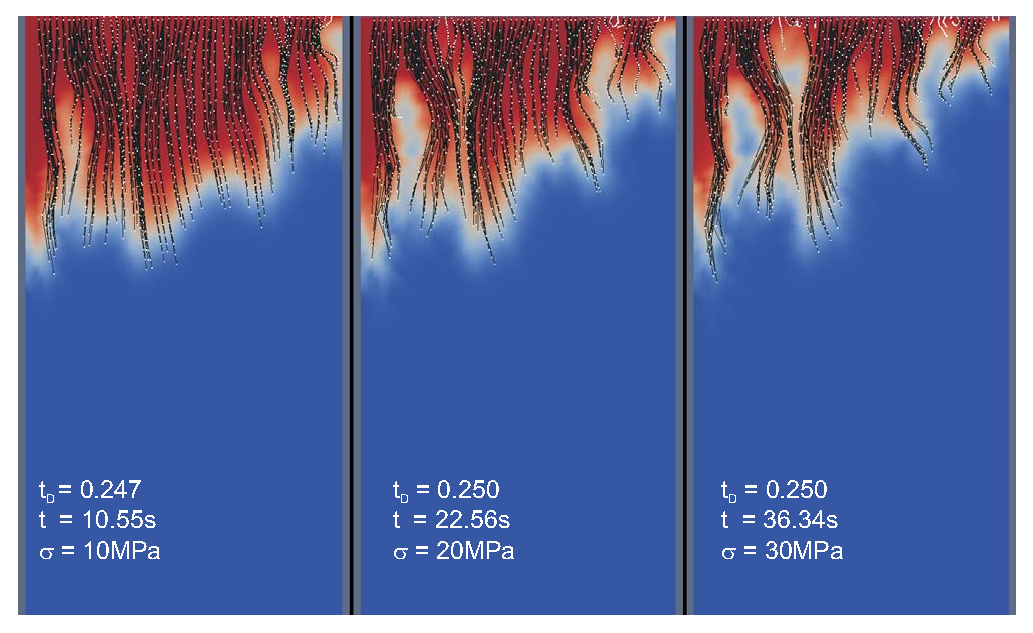
\includegraphics[width=0.8\textwidth]{PART_II/C/rwptfrac.eps}
\caption{RWPT vs. ADE at different stress states. Two separate simulations are conducted and overlay one another. Particle pathlines (black) and particles (white) are illustrated, and overlay contours (red = higher concentration) generated from the ADE simulation.}
\label{fig:stress_rwpt}
\vspace{5mm}
\end{figure}